\documentclass[UTF8]{ctexbeamer}

\input{header.tex}

%-------------title here--------------------
\title{Implantation d'un parseur et d'un jeu d'instructions pour le langage CHIPS}
% \subtitle{Projet de Développement Agile de Machines Virtuelles}
\course{Master 2 Informatique}
\author{\vspace{-5}Anton DOLARD, Vital FOCHEUX, Julien GAUTHIER \\
        Tutrices : Anna GALLONE, Olga KOUCHNARENKO}
\IDnumber{}

\usepackage{listings}
\lstdefinelanguage{Chips}{
  morekeywords={logical, physical,object,system,init,then,spread,collect,as,with,implementation,input,stop,among,ctx,using,actuator,sensor},
  sensitive=true,
  morecomment=[l]{//},
  morestring=[b]"
}
\lstset{
  basicstyle=\ttfamily\small,
  keywordstyle=\color{blue}\bfseries,
  commentstyle=\color{gray},
  stringstyle=\color{red!60!black},
  showstringspaces=false,
  columns=fullflexible,
  frame=single,
  breaklines=true
}

\date{26 février 2026}
%--------------begin document--------------------
\begin{document}
\maketitle

\themecolor{main}
\footlinecolor{}
\begin{frame}[noframenumbering]{}
    \framesubtitle{Plan de la présentation}
    \tableofcontents
\end{frame}
\themecolor{}

% Start of the presentation
\footlinecolor{maincolor}
\setbeamercolor{block body}{fg=darkgray,bg=ufcgrey}

\section{Introduction}
\begin{frame}{Présentation CHIPS}
    \begin{block}{Présentation CHIPS}
        \begin{itemize}
            \item Langage de modélisation de systèmes distribués et embarqués
            \item Représente les applications distribuées sous la forme de deux graphes:
            \begin{itemize}
                \item Graphe fonctionnel (nœuds $\rightarrow$ algorithmes, arêtes $\rightarrow$ flux de données)
                \item Graphe de dépendance physique (nœuds $\rightarrow$ algorithmes, arêtes $\rightarrow$ dépendances matérielles)
            \end{itemize}
            \item Compilation vers un modèle formel (XMI puis BIP)
        \end{itemize}
    \end{block}
\end{frame}

\begin{frame}{Motivations}
   \begin{block}{Objectifs du projet}
        \begin{itemize}
            \item Langage récent
            \item Certaines constructions syntaxiques ne sont pas encore prises en charge
            \item Gestion des erreurs
            \item Sérialisation de l'AST vers le format XMI
            \item Implémentation d'un Grammar Based Testing (GBT)
        \end{itemize}
    \end{block}
\end{frame}

\begin{frame}{Technologies utilisées}
    \begin{block}{Technologies utilisées}
        \begin{itemize}
            \item Flex et Yacc $\rightarrow$ parser
            \item C++ et XMI $\rightarrow$ parser et sérialisation
            \item Python $\rightarrow$ validation XMI et GBT
            \item GitHub $\rightarrow$ gestionnaire de versions
            \item Notion $\rightarrow$ gestion des tâches
            \item Discord $\rightarrow$ communication
        \end{itemize}
    \end{block}
\end{frame}

\section{Algorithmes et technologies}
\subsection{Lexer et Parseur}

\begin{frame}{Lexer}
    
    \hspace{-5mm}

    \begin{block}{La création}
        \begin{itemize}
            \item Définition d'expressions régulières pour certains jetons :
            \begin{itemize}
                \item DIGIT [0-9] 
                \item IDENT [a-zA-Z][a-zA-Z0-9\_]*
            \end{itemize}
            \item Création de jetons pour les symbôles terminaux $\longrightarrow$ +, physical, system \dots
        \end{itemize}
    \end{block}
    
    \begin{block}{Jetons existants}
        \begin{itemize}
            \item Opérateurs binaires et unaires
            \item Littéraux
            \item Types de données et types de fonctions
            \item Jetons spécifiques à CHIPS
            \item Jetons existants dans d'autres langages
        \end{itemize}
    \end{block}
\end{frame}

\begin{frame}{Parseur}

    \hspace{-5mm}

    \begin{figure}
        \centering
        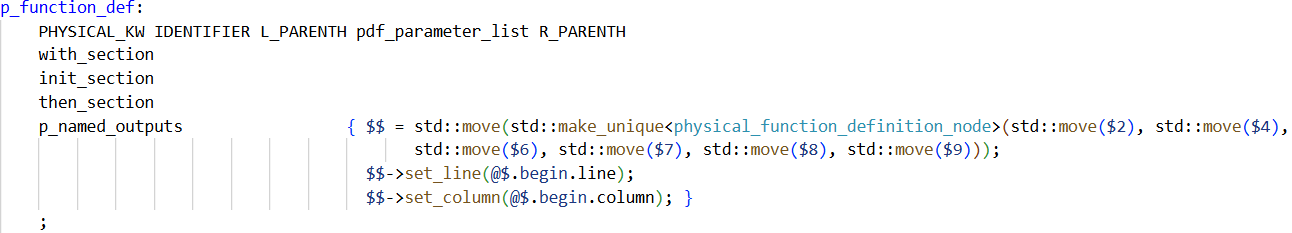
\includegraphics[width=\textwidth]{img/grammar.png}
        \caption{Exemple d'une règle de grammaire}
        \label{fig:grammaire_physical}
    \end{figure}
    
    \begin{block}{Fonctionnement}
        \begin{itemize}
            \item Déclaration des règles $\longrightarrow$ utilisation de jetons terminaux/non-terminaux
            \item Création des noeuds de l'AST
            \item Affectation du numéro de la ligne et la colonne $\longrightarrow$ pour les erreurs
        \end{itemize}
    \end{block}
\end{frame}


\subsection{Sérialisation vers XMI}

\begin{frame}{Passage de l'AST au modèle XMI}
    \begin{itemize}
        \item \textbf{Pourquoi le format XMI ? :}
        \begin{itemize}
            \item Standard de l'OMG pour l'échange de métadonnées.
            \item Interopérabilité avec \textbf{EMF} (Eclipse Modeling Framework).
        \end{itemize}
        \vfill
        \item \textbf{Qu'est-ce que le Méta-modèle CHIPS (Ecore) ? :}
        \begin{itemize}
            \item Définit la "grammaire" stricte du modèle (entités, relations).
            \item Utilisation des schémas \texttt{chips1.1.ecore} ou \texttt{chips2.ecore}.
        \end{itemize}
        \vfill
        \item \textbf{Comment valider le format ? :}
        \begin{itemize}
            \item Garantie de conformité via un script de validation basé sur EMF (\texttt{xmi\_validator.py}).
        \end{itemize}
    \end{itemize}
\end{frame}

\begin{frame}{Transformation et parcours de l'AST}
    \begin{columns}
        \begin{column}{0.6\textwidth}
            \begin{itemize}
                \item \textbf{ChipsToXmiVisitor :}
                \begin{itemize}
                    \item Parcours récursif de l'AST.
                    \item Génération dynamique du flux XML.
                \end{itemize}
                \item \textbf{Gestion du contexte :}
                \begin{itemize}
                    \item \texttt{m\_currentPath} : Maintien de la position hiérarchique (ex: \texttt{//@preamble/@definitions.0}).
                    \item Construction incrémentale des fragments d'URI.
                \end{itemize}
                \item \textbf{ChipsToXmiWriter :} Reprend la sortie du visiteur et sépare le corps du XMI (\texttt{bodywriter}) et les en-tête pour gérer dynamiquement les \textit{namespaces}.
            \end{itemize}
        \end{column}
        \begin{column}{0.4\textwidth}
            \centering
            \textbf{Flux de données}
            \vspace{0.5cm}
            \begin{exampleblock}{Pipeline}
                Code CHIPS \\
                $\downarrow$ \\
                AST (C++) \\
                $\downarrow$ \\
                \textbf{Visiteur XMI} \\
                $\downarrow$ \\
                Modèle XMI
            \end{exampleblock}
        \end{column}
    \end{columns}
\end{frame}

\begin{frame}{Résolution des liens et gestion des symboles}
    \begin{itemize}
        \item \textbf{Problématique :} Faire le lien entre un \textit{nom} (code source) et un \textit{chemin relatif} (XMI).
        \item \textbf{Solution :} Une table des symboles double.
        \begin{itemize}
            \item \texttt{m\_symbolTable} : Lie un identifiant à son chemin XMI définitif.
            \item \texttt{m\_definitionsTable} : Gère les variables locales (\texttt{with}, \texttt{init}, \texttt{then}).
        \end{itemize}
    \end{itemize}
\end{frame}

\begin{frame}[fragile]{Exemple de résolution 1/5}
  Voici la définition du sous-composant logique :
  \begin{figure}
        \centering
        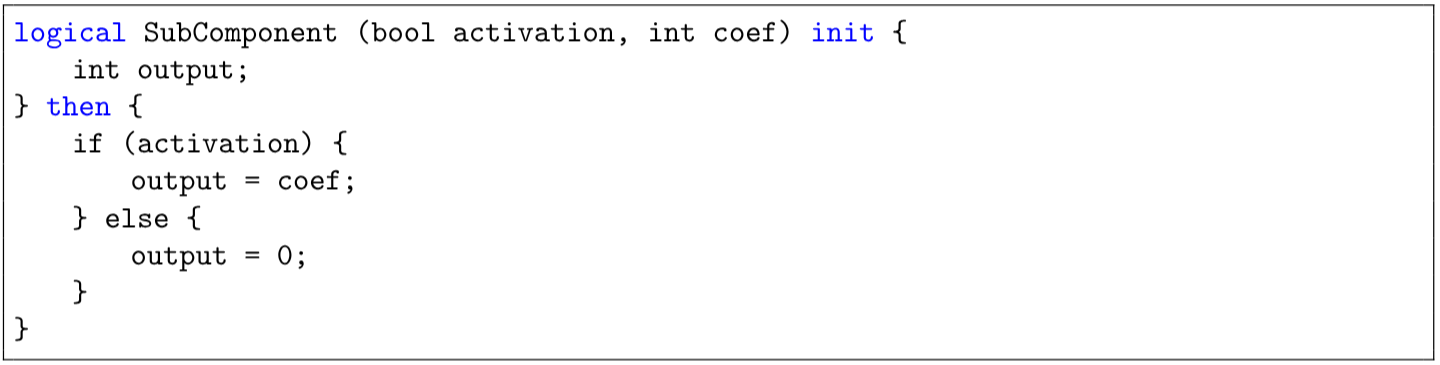
\includegraphics[width=\textwidth]{img/exemple_chips.png}
        \caption{Exemple d'un composant logique en CHIPS}
        \label{fig:logical_component}
    \end{figure}
\end{frame}

\begin{frame}[fragile]{Exemple de résolution 2/5}
    \begin{figure}
        \centering
        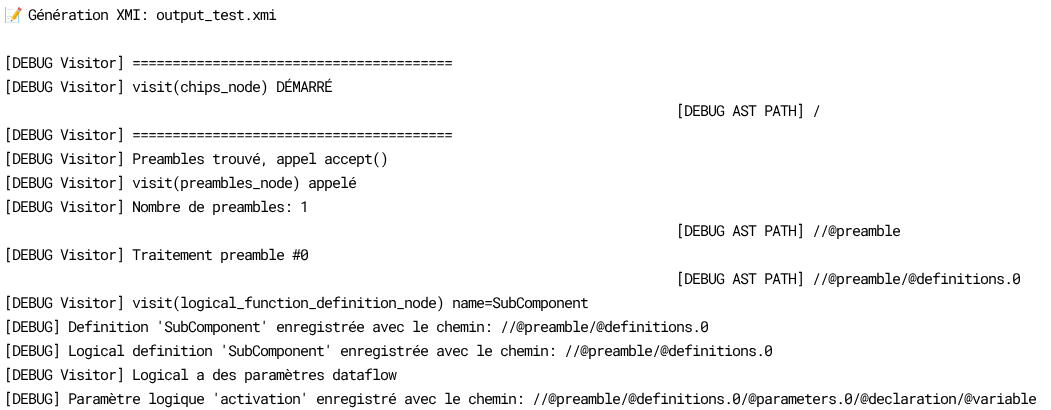
\includegraphics[width=\textwidth]{img/debug_message.png}
        \caption{Extrait des messages de debogage pour la génération XMI}
        \label{fig:xmi_debbug}
    \end{figure}
\end{frame}

\begin{frame}[fragile]{Exemple de résolution 3/5}
    \begin{figure}
        \centering
        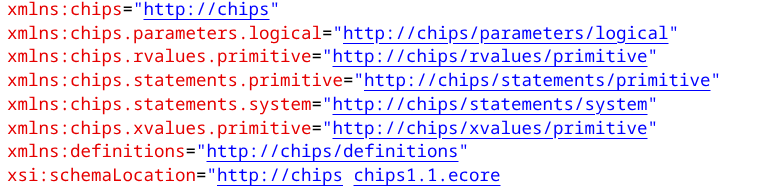
\includegraphics[width=\textwidth]{img/namespace.png}
        \caption{Extrait des namespaces générés}
        \label{fig:xmi_namespace}
    \end{figure}
\end{frame}

\begin{frame}[fragile]{Exemple de résolution 4/5}
  \begin{figure}
        \centering
        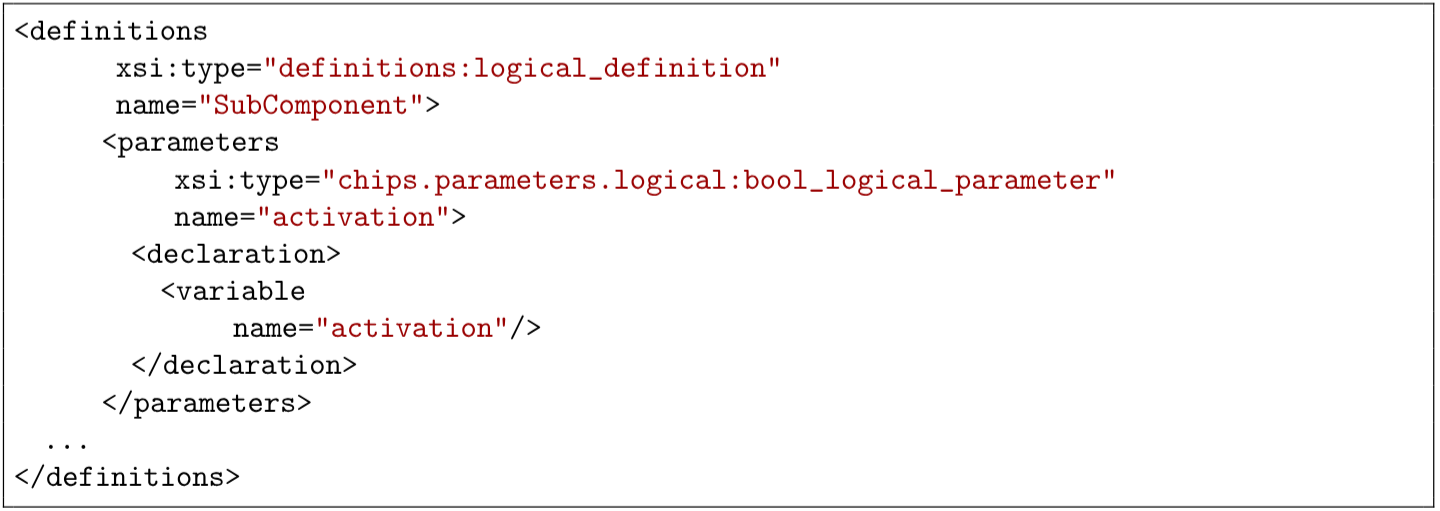
\includegraphics[width=\textwidth]{img/exemple_xmi.png}
        \caption{Extrait de la génération XMI du composant logique}
        \label{fig:xmi_writing}
    \end{figure}
\end{frame}

\begin{frame}[fragile]{Exemple de résolution 5/5}
  \begin{figure}
        \centering
        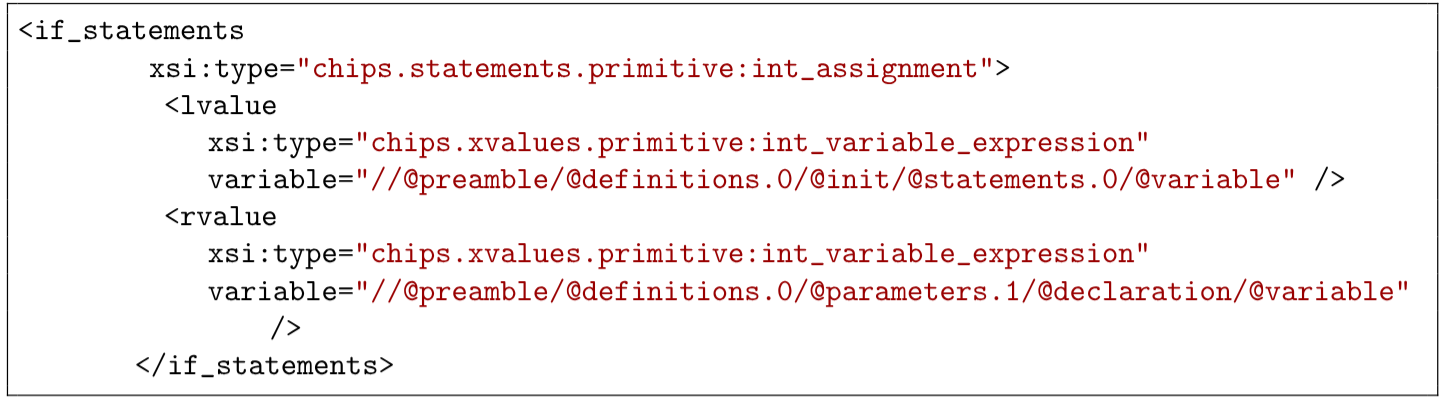
\includegraphics[width=\textwidth]{img/exemple_xmi_2.png}
        \caption{Extrait de la génération XMI du composant logique}
        \label{fig:xmi_writing_2}
    \end{figure}
\end{frame}

\section{Conformité du langage}

\subsection{Vérification du XMI}
\begin{frame}{XMIValidator.py}
    \begin{block}{Explications}
        \begin{itemize}
            \item Programme Python de validation XMI basé sur PyEcore
            \item Vérification qu’un fichier XMI respecte un métamodèle Ecore
            \item Chargement automatique du métamodèle et de ses sous-packages
            \item Validation de la structure et détection des erreurs
        \end{itemize}
    \end{block}
\end{frame}
\subsection{Grammar Based Testing}

\begin{frame}{Le Grammar Based Testing c'est quoi ?}
    \begin{block}{Explications}
     Le Grammar Based Testing (GBT) consiste à :
        \begin{itemize}
            \item Générer automatiquement des programmes valides à partir de la grammaire du langage
            \item Vérifier que le compilateur accepte ces programmes valides
            \item Modifier certains programmes pour créer des erreurs syntaxiques (mutants)
            \item Vérifier que le compilateur renvoie bien une erreur pour ces programmes invalides
        \end{itemize}
    \end{block}
\end{frame}

\begin{frame}{Comment on génère ?}
    \begin{block}{Programmes valides}
        \begin{itemize}
            \item On construit un fichier .chips de haut en bas.
            \item On génère d’abord les préambules : logical, physical, object, implementation.
            \item On génère ensuite un bloc SYSTEM \{...\}.
            \item Dans SYSTEM, le programme choisit une liste d’instructions valides.
            \item La profondeur est limitée afin de garantir la terminaison.
        \end{itemize}
    \end{block}
\end{frame}
\begin{frame}{Comment on génère ?}
    \begin{block}{Programmes invalides}
        \begin{itemize}
            \item On part d'un programme valide et on applique une mutation locale
            \item Exemples : suppression de { ;}, {\{}, {\}}, {( )}, {[ ]}, insertion de tokens parasites, altération de mots-clés, etc.
            \item Le générateur garantit que toutes les catégories de mutations sont présentes
        \end{itemize}
    \end{block}
\end{frame}

\begin{frame}{La vérification automatique}
    \begin{block}{run\_gbt\_valid}
        \begin{itemize}
            \item Parcourt le dossier \texttt{ShouldCompileSyntax/}
            \item Exécute le compilateur sur tous les fichiers
            \item Si la compilation échoue $\rightarrow$ erreur
            \item Affiche le nombre total d'échecs
        \end{itemize}
    \end{block}

    \begin{block}{run\_gbt\_invalid}
        \begin{itemize}
            \item Parcourt le dossier \texttt{ShouldNotCompileSyntax/}
            \item Exécute le compilateur sur tous les fichiers
            \item Si la compilation réussit $\rightarrow$ validation inattendue
            \item Affiche le nombre total de validations inattendues
        \end{itemize}
    \end{block}
\end{frame}

\begin{frame}{Résultats}
    \begin{block}{500 fichiers valides, 500 fichiers invalides}
        \begin{itemize}
            \item 0 erreurs inattendues
            \item 0 validations inattendues
            \item Toutes les mutations apparaissent au moins une fois
            \item 182 règles apparaissent en réduction
        \end{itemize}
    \end{block}
\end{frame}

\subsection{Les erreurs syntaxiques}

\begin{frame}[fragile]{Syntaxe}

    \begin{figure}
        \centering
        \begin{verbatim}
            physical test()
            init{
                int x = 0
            } -> output()
        \end{verbatim}
        \caption{Exemple erreur de syntaxe}
    \end{figure}

    \begin{block}{Fonctionnement}
        \begin{itemize}
            \item Le parseur gère le non respect de la syntaxe
            \item Il émet une erreur $\longrightarrow$ syntax error, unexpected R\_CURL, expecting SEMICOL
        \end{itemize}
    \end{block}
\end{frame}

\subsection{Les erreurs sémantiques}

\begin{frame}{Sémantique de base}
    \begin{block}{Fonctionnement}
        Durant le parcours de l'AST, on utilise une table des symbôles pour :
        \begin{itemize}
            \item Garder en mémoire les variables et fonctions déclarées
            \item Lever des erreurs par moment $\longrightarrow$ variable redéclarée, utilisation de variable non déclarée \dots
        \end{itemize}
    \end{block}
\end{frame}

\begin{frame}{Sémantique plus avancée}
    \begin{block}{Graphe dirigé acyclique}
        % Utilisation d'un graphe dirigé acyclique qui a :
        \begin{itemize}
            \item Sommet $\longrightarrow$ des fonctions physique ou logique
            \item Arrête $\longrightarrow$ le lien entre ces fonctions lors de l'instruction link
        \end{itemize}
        
    \end{block}
        
    \begin{block}{Vérification}
        \begin{itemize}
            \item Que les fonctions de source et/ou cible existe
            \item Qu'une fonction physique n'est jamais la source
            \item Qu'il n'y a pas de cycle dans le graphe final $\longrightarrow$ problème de dépendance (A $\xrightarrow{}$ B $\xrightarrow{}$ C $\xrightarrow{}$ A)
        \end{itemize}
    \end{block}
\end{frame}

\begin{frame}{Exemple de dépendance}
    \begin{columns}[c]
    
    \column{0.3\textwidth}
    \centering
    
\includegraphics[width=\linewidth]{img/pistons.png}
    
    \column{0.05\textwidth}
    \centering
    $\rightarrow$
    
    \column{0.3\textwidth}
    \centering
    
\includegraphics[width=\linewidth]{img/moteur.png}
    
    \column{0.05\textwidth}
    \centering
    $\rightarrow$
    
    \column{0.3\textwidth}
    \centering
    
\includegraphics[width=\linewidth]{img/voiture.png}
    
    \end{columns}
\end{frame}

\section{Conclusion}
\subsection{Bilan technique}

\begin{frame}{Bilan}
\begin{block}{Réalisation effectuée}
    \begin{itemize}
        \item Lexer et parser opérationnels
        \item Pipeline complet CHIPS $\xrightarrow{}$ AST $\xrightarrow{}$ XMI (sous-ensemble du langage)
        \item Modèle GBT $\xrightarrow{}$ production de tests d'acceptations
    \end{itemize}
\end{block}

\begin{block}{Réalisation pour le futur}
    \begin{itemize}
        \item Finir la sérialisation de l'AST vers XMI en entier
    \end{itemize}
\end{block}
\end{frame}

\subsection{Bilan personnel}

\begin{frame}{Bilan}

\begin{block}{Gestion de projet et ressentit}
    \begin{itemize}
        \item Prise d'initiative (ex: GBT)
        \item Capacité d'adaptation
        \item Mise en lien avec les cours de \textbf{Systèmes Cyber-Physiques (M2)} et \textbf{Validation à Base de Modèles (M2)} 
    \end{itemize}
\end{block}
    
\end{frame}

\begingroup
  \themecolor{main}
  \begin{frame}[c]
    \centering
    \begin{minipage}{\textwidth}
      \usebeamercolor[fg]{normal text}
      \centering
      \Huge \textsl{Merci de votre attention ! } \\
      \Huge \textsl{Des questions ?}
    \end{minipage}
  \end{frame}
\endgroup
\end{document}